\documentclass[11pt, a4paper, openany]{article}
\usepackage{geometry}
 \geometry{
 a4paper,
 left=2.0in,
 right=1.0in,
 top=1.5in,
 bottom=1.0in
 }
\usepackage[utf8]{inputenc}
\usepackage[nottoc,numbib]{tocbibind}
\usepackage{graphicx}
\usepackage{amsmath}
\usepackage{subfig}
\usepackage{url}
\usepackage{float}
\usepackage{booktabs} % Allows the use of \toprule, \midrule

\graphicspath{ {files/} }
\newcommand*{\SignatureAndDate}[1]{%
    \par\noindent\makebox[2.5in]{\hrulefill} \hfill\makebox[2.0in]{\hrulefill}%
    \par\noindent\makebox[2.5in][l]{#1}      \hfill\makebox[2.0in][l]{Date}%
}%
\usepackage{titlesec}
\usepackage{fancyhdr}

\begin{document}
\pagenumbering{gobble}% Remove page numbers (and reset to 1)
\begin{center}
{\Huge Final Year Project}
\end{center}
\vspace{.2in}
\begin{center}
{\Huge Reconstruct3D}
\end{center}
\vspace{.15in}
\begin{center}
{\huge Analysis of Structure from Motion Techniques}
\end{center}
\vspace{.5in}
\begin{center}
{\Large Group members}
\end{center}
\vspace{.10in}
\begin{center}
{\large Muneeb Aadil (14I-0140)}
\end{center}
\begin{center}
{\large Adeel Ahmad (14I-0169)}
\end{center}
\vspace{.7in}
\begin{center}
{\Large Supervised by}
\end{center}
\vspace{.10in}
\begin{center}
{\large Dr. Sibt ul Hussain}
\end{center}
\vspace{.6in}
\begin{center}
{\large Department of Computer Science}
\end{center}
\vspace{.10in}
\begin{center}
{\large National University of Computer and Emerging Sciences}
\end{center}
\vspace{.10in}
\begin{center}
{\large Islamabad, Pakistan}
\end{center}
\vspace{.10in}
\begin{center}
{\large 2018}
\end{center}
\mbox{} \
\vfill \
\begin{center}
\noindent\rule{14cm}{0.4pt}
\end{center}
\newpage

\pagestyle{fancy}
\fancyhf{}

\fancyhead[L]{\ifodd\value{page}Analysis of Structure from Motion Techniques\else \rightmark\fi}
\fancyhead[R]{\thepage}
\fancyhead[R]{\ifodd\value{page}\fi \thepage}

\pagenumbering{roman}

\noindent\textbf{Authors' Submission} \\

We hereby declare that the work presented in this report is our own work. All the references are properly cited, wherever they are used in the document.\\
\newline
\newline
\newline
\textbf{Abstract} \\
\newline
To reconstruct a 3D model/mesh, one requires dedicated hardware such as depth-enabled cameras (i.e. RGBD cameras) or stereoscopic cameras. Such hardware is not available within general purpose smartphones and hence this technology is not accessible for the general public. In this project, we aim to reconstruct a 3D model of static scenery from a monocular video sequence.

To start off with the reconstruction process, a user captures a video of the real 3D world. Then, this video is transferred to a remote server for computation of its 3-dimensional model (which is to be done using epipolar geometry techniques). After the server has finished its computation, user can download the reconstructed 3D model of the static environment.

The main steps in this project include feature matching, fundamental matrix estimation, camera pose estimation, triangulation, perspective-n-point, and depth map estimation. Finally, we present a metric for quantifying our results.\\

\newpage
\noindent\textbf{Executive Summary} \\
\newline
The report focuses on the problem of generating 3D structure from a set of 2D images. This work is intended to remove the literature barrier of introductory knowledge in the domain of 3D vision, by providing concise yet sufficient and complete resources containing the source code, reference results to cross-check other against implementations, and theoretical foundations. \newline

Firstly, we explain the importance of this problem by listing out some of the applications areas where this problem is faced. We also take a look on the challenges commonly faced while designing a robust solution to give us an idea of the difficulty of the problem. Furthermore, we formalize the problem by expressing our objective in mathematical notation. \newline

Having formalized the problem, we then explain the theoretical foundations of 3D vision necessary for understanding standard pipelines of structure from motion. More specifically, we explain (1) a single view geometry: a transformation governing the process of capturing data from 3D world to 2D camera, (2) multi-view geometry: a set of geometric relations that exist between two cameras capturing the same 3D scene from different angles at the same time, (3) process of actually projecting 2D data back to 3D space once we have the necessary entities, and (4) some miscellaneous topics such as matching corresponding points between two images of the same scene, removing outliers for robust computation, etc. \newline

Armed with theoretical foundations, we provide a complete algorithm from theoretical and implementation perspective. We list the major tools and libraries we used in our implementation. We also provide a web interface for users to upload the images and view the results online. \newline

Lastly, we apply our implementation to variety of datasets including standard benchmarks and provide qualitative and quantitative results of each dataset along with the effect on each hyper-parameter on final performance. We also comment on future directions that can be taken to further enhance reproducible research by implementing other pipelines of structure from motion.
\newpage

\tableofcontents
\newpage
\pagenumbering{arabic}

\titleformat*{\section}{\LARGE\bfseries}


\section{Introduction}
3D reconstruction from video has been an active research area in Computer Vision for the past few years. Some of this research also overlaps with Digital Photogrammetry \cite{photogrammetry}, which involves estimating measurements from photographs. It finds extensive applications in numerous domains, such as medical imaging, robotics, computer graphics, virtual reality etc. This greatly reduces the effort required to assemble a digital map. A user could simply provide an extensive video of an area/scene and obtain the end result through an automated process. Recent applications include virtual tours of cities, tourism, and city planning.

\subsection{Problem Domain} In the past, reconstruction was performed using photogrammetric techniques, in which images were manually processed. Due to a large amount of available data, this was a highly expensive and time consuming process. Therefore, this process had to be automated.

The proposed reconstruction process involves several stages, ranging from low-level to high-level processing \cite{reconstruction steps}. A state of the art system would depend on the success of all these stages and in combining the end result. This process is made difficult from the fact that a lot of information is lost as images are projected to 3D space. Apart from this, we have to filter out the useful information and discard all irrelevant details.

\subsection{Research Problem Statement} Given a video sequence of static environment, the task is to compute its 3D model/mesh. This problem can be formalized as follows:
given $m$ pixels in $n$ images $x_{11}, x_{12}\ldots x_{1n}, x_{21}\ldots x_{2n}, x_{m1}\ldots x_{mn}$, compute the camera projection matrix $P_{1}, P_{2}\ldots P_{n}$ for each image and 3D coordinates of each point $X_{1}, \dots X_{m}$ such that each 2D point-correspondences\footnote{2D Point Correspondences: Set of 2D points, each in different image, which corresponds to the same point in 3D world.} across the images projects to one 3D scene point. This is known as \textbf{re-projection error} and its definition is as follows:

\begin{center} $E = \sum_{j}^{m} \sum_{i}^{n}\begin{Vmatrix}
x_{j} - P_{i}X_{j}
\end{Vmatrix}^{2}$ \end{center}

The goal is to find a set of camera projection matrices $P_{1}, P_{2}\ldots P_{n}$, and 3-dimensional coordinates of each point $X_{1}, \dots X_{m}$ that minimize the re-projection error:
\begin{center} $\min_{P_{1},\dots P_{n}, X_{1},\ldots X_{m}} E$ \end{center}


\section{Literature Review}
The following sections explain, in detail, the technicalities that deal with reconstruction of 3D environment from 2D images. The algorithms provided in these sections are explained using mathematical equations. Additional reading material is cited for a more in-depth understanding.

\subsection{Camera Projections} The camera model is responsible for transforming the visual representation of real 3D world into 2D camera pixels \cite{camera model}, \cite{camera model2}. As shown in Figure \ref{fig:cameraprojs}, the camera projection matrix $P$ projects the world coordinate system into image plane i.e. pixel coordinate system which lies at $z = 1$.

\begin{figure}
  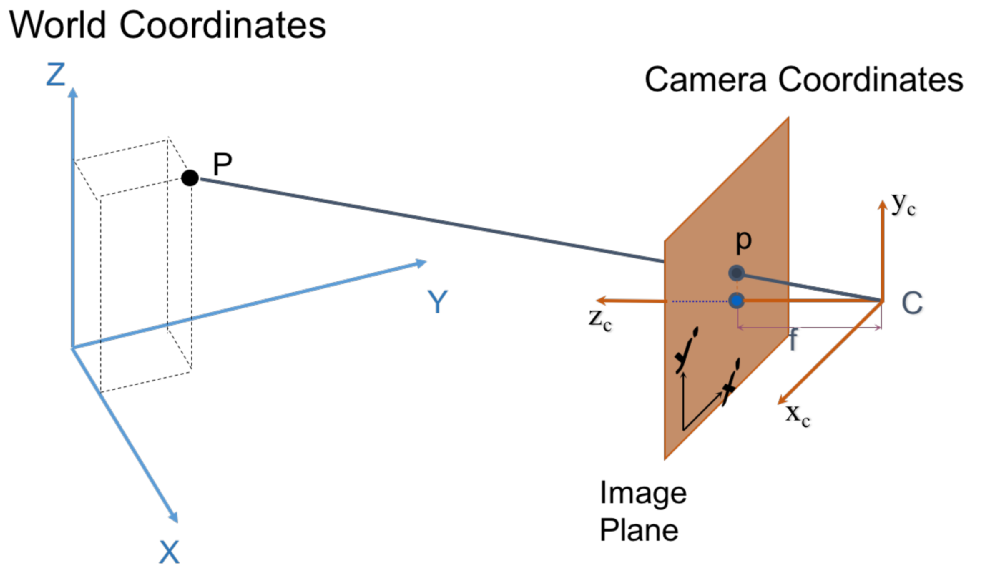
\includegraphics[width=\linewidth]{transformation.png}
  \caption{Camera Projections}
  \label{fig:cameraprojs}
\end{figure}

Mathematically, the projection matrix $P$ is a $3\times4$ matrix which can be further decomposed into two matrices as shown below:
\begin{center}$P = K[R|t]$\end{center}
Where $[R|t]$ and $K$ denote the extrinsic and intrinsic camera parameters, respectively. They are briefly explained below:
\begin{itemize}
\item \textbf{Extrinsic Parameters} are denoted by a $3\times4$ matrix ($3\times3$ Rotation Matrix $R$ concatenated with $3\times1$ Translation Vector $t$). Rotation matrix and translation vector encodes the camera orientation and position (w.r.t world coordinate frame), respectively. Collectively, it transforms 3D world in third person view to first person view. Note that transformation occurs in coordinate space and not the pixel space.
\item \textbf{Intrinsic Parameters} are denoted with a $3\times3$ matrix K which encodes camera's internal properties, such as, lens'  focal length, principal point, pixel scaling factor etc. It transforms the 3D world in first person view (provided by extrinsic transformation) to 2D pixel in first person view.
\end{itemize}
Now, given a projection matrix $P$ and point $X$ in 3D world coordinate system, it is mapped to a 2D pixel coordinate system $x$ using the following relation:
\begin{center}$x = \overset{P}{\overbrace{K[R|t]}}X$\end{center}

\subsection{Camera Calibration and Pose Estimation} To determine the camera calibration, several parameters, such as focal length, optical center, and aspect ratio need to be known. There are numerous approaches through which we can estimate the camera pose, such as  linear regression, vanishing points, and panoramas. The end result is the calibration matrix, denoted by $KX_{c}$.\newline
Once the internal camera parameters are known, we can then compute camera pose. The two mostly used methods are: vanishing points and planar pattern. After applying one these techniques to compute the camera pose, we can superimpose it on our original image.

\subsection{Epipolar Geometry and the Fundamental Matrix} Given two views/images, epipolar geometry is essentially the geometry of intersection between them \cite{section 9.1}. For example, when a 3D point $X$ is imaged in two views $x$ and $x'$, the camera centers $C$ and $C'$, image points $x$ and $x'$, and 3D point $X$ lie in the same plane, as shown in Figure \ref{fig:epipolar}(a). These geometry principles aid in constraining our search space for finding point correspondences.\newline

\begin{figure}%
    \centering
    \subfloat[The camera centres, 3-space point $X$, and its images $x$ and $x'$ lie in a common
plane]{{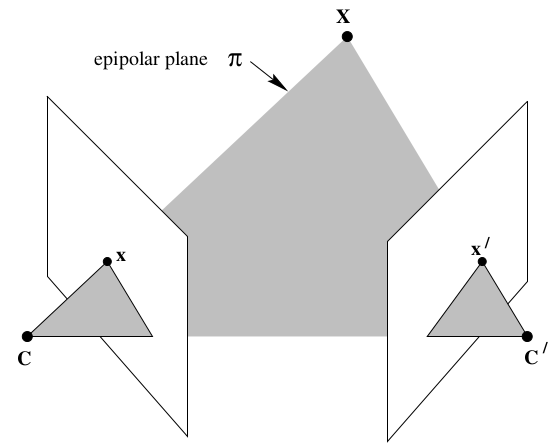
\includegraphics[width=6cm]{epipolargeo.png} }}%
    \qquad
    \subfloat[The camera baseline intersects each image plane at the epipoles $e$
and $e'$]{{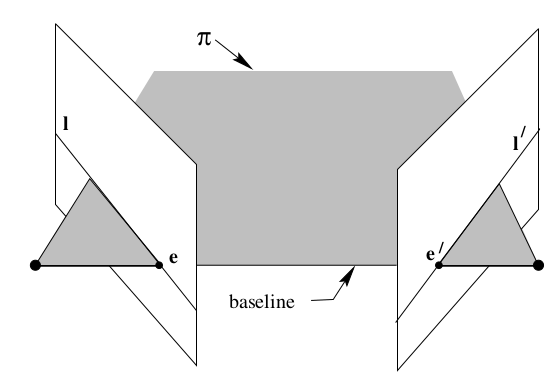
\includegraphics[width=6cm]{epipolargeo-2.png} }}%
    \caption{Epipolar Geometry}%
    \label{fig:epipolar}%
\end{figure}

A few fundamental terminologies of epipolar geometry are defined as following:
\begin{itemize}
\item \textbf{Epipole} $e$ is the point of intersection of the line joining the camera centres with the image plane (see Figure \ref{fig:epipolar}(b)).
\item \textbf{Epipolar Plane} $\pi$ is a plane containing the baseline. There is a one-parameter
family (a pencil) of epipolar planes.
\item \textbf{Epipolar Line} $l$ is the intersection of an epipolar plane with the image plane. All epipolar lines intersect at the epipole (see Figure \ref{fig:epipolar}(b)).
\end{itemize}
The fundamental matrix $F$ is a 2-rank $3\times3$ matrix which represents epipolar geometry. It describes the geometric relations that exist between two images of the same scene, and is estimated by the number of correspondences between them. A correspondence is a pair of points on the two images that are believed to be projections of the same 3D point. Fundamental matrix $F$ satisfies what's called a Correspondence Condition \cite{fundamentalcorrespondingcondition}. It is stated as follows: \newline
The fundamental matrix satisfies the condition that for any pair of corresponding points $x \leftrightarrow x'$ in the two images
\begin{center}$xFx' = 0$\end{center}

\subsection{8 Point Algorithm for Fundamental Matrix Estimation} \label{8pointsec} As explained above and in \cite{8point}, for all point correspondences $x$ and $x'$, It satisfies the following equation:
\begin{center}
$x'^{T}Fx=0$
\end{center}
Expanding and rearranging this equation yields the following formulation:
\begin{equation}\label{eq1}
Ax = 0
\end{equation}
where
\begin{center}
$A = \begin{bmatrix}  u_{1}^{(1)}u_{1}^{(2)}  \hspace{5mm} u_{1}^{(1)}u_{1}^{(2)} \hspace{5mm} u_{1}^{(1)}  \hspace{5mm} v_{1}^{(1)}u_{1}^{(2)}  \hspace{5mm} v_{1}^{(1)}v_{1}^{(2)}  \hspace{5mm} v_{1}^{(1)} \hspace{5mm} u_{1}^{(2)} \hspace{5mm} v_{1}^{(2)} \hspace{5mm} 1\\   -- \hspace{5mm}  -- \hspace{5mm}  -- \hspace{5mm}  -- \hspace{5mm}  -- \hspace{5mm}  -- \hspace{5mm}  -- \hspace{5mm}  \\   u_{8}^{(1)}u_{8}^{(2)}  \hspace{5mm} u_{8}^{(1)}u_{8}^{(2)} \hspace{5mm} u_{8}^{(1)}  \hspace{5mm} v_{8}^{(1)}u_{8}^{(2)}  \hspace{5mm} v_{8}^{(1)}v_{8}^{(2)}  \hspace{5mm} v_{8}^{(1)} \hspace{5mm} u_{8}^{(2)} \hspace{5mm} v_{8}^{(2)} \hspace{5mm} 1  \end{bmatrix}$\\[10pt]
$x = \begin{bmatrix} f_{11}&f_{12}&f_{13}&f_{21}&f_{22}&f_{23}&f_{31}&f_{32}&f_{33}\\ \end{bmatrix}^T$\\[10pt]
$u_{i}^{k}$ = x-coordinate of ith point in kth image\newline
$v_{i}^{k}$ = y-coordinate of ith point in kth image\newline
$f_{i}^{j}$ = ith row, jth column entry of matrix $F$\newline
\end{center}

The algorithm consists of the following steps:
\begin{description}
\item \textbf{8 Corresponding Points} First, a total of eight 2D point correspondences between images are determined.

\item \textbf{SVD (Singular Value Decomposition)} To solve equation (\ref{eq1}), we compute SVD of matrix $A = UDV^{T}$ and reshape the last column of $V$ into a $3\times3$ matrix which represents the fundamental matrix $F'$. (See Appendix A for more details.)

\item \textbf{Applying Rank Constraint} The fundamental Matrix $F'$ computed in the last step will not necessarily have rank 2 (which is one of the requirements for a valid fundamental matrix) due to noise present in the data. Thus, we now compute SVD of $F' = UDV^{T}$ and explicitly reduce the rank to 2 by setting the last diagonal element of $D$ to zero to get $D'$. Finally, we get a valid fundamental matrix $F = UD'V^{T}$.
\end{description}

\subsection{Essential Matrix and Extraction of Camera Matrices} The essential matrix is the specialization of the fundamental matrix to the case of normalized image coordinates. In fundamental matrix the assumption of calibrated cameras is removed, so it can be thought of as a generalization of the essential matrix. The essential matrix can be directly computed from the fundamental matrix using equation (\ref{essfund}) from which the camera projection matrix is further computed \cite{section 9.6}, \cite{pose estimation}.

\begin{equation}\label{essfund}
E = K'^{T}FK
\end{equation}

For a computed essential matrix $E = U diag(1, 1, 0)V^{T}$, and first camera matrix $P = [ I | 0 ]$, there are four possible choices for the second camera matrix $P'$
\begin{center}
$P' = [UWV^{T}| + u_{3}]$\newline
$P' = [UWV^{T}| - u_{3}]$\newline
$P' = [UW^{T}V^{T}| + u_{3}]$\newline
$P' = [UW^{T}V^{T}| - u_{3}]$\newline
\end{center}
where
\begin{center}
$u_{3}$ = Third column of matrix $U$\newline
$W$ = $\begin{bmatrix}
0 & -1 & 0\\
1 & 0 & 0\\
0 & 0 & 1
\end{bmatrix}$ \newline
\end{center}

\subsection{Triangulation} Triangulation is a problem of estimating a 3D point $X$, given its point correspondences $x_{1}, x_{2}, \ldots , x_{n}$ and camera matrices $P_{1}, P_{2}, \ldots , P_{n}$ computed for each image $I_{1}, I_{2}, \ldots I_{n}$ \cite{triangulation}. There are generally two approaches followed to solve this problem: Linear and Nonlinear; both of which are explained below:
\begin{figure}[!ht]%
    \centering
    \subfloat[Ideal Case]{{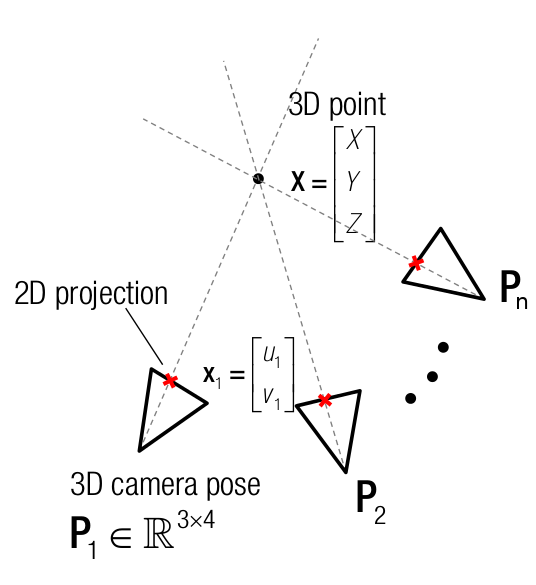
\includegraphics[width=6cm]{triangulate1.png} }}%
    \qquad
    \subfloat[Pratical Case]{{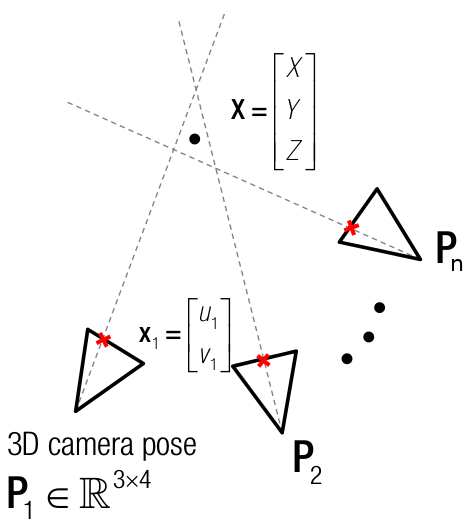
\includegraphics[width=6cm]{triangulate2.png} }}%
    \caption{Triangulation Setups}%
    \label{fig:triangulation}%
\end{figure}

\begin{description}
\item \textbf{Linear Triangulation:} As the name suggests, linear triangulation tackles this problem assuming a linear relationship between the variables since, as shown in Figure \ref{fig:triangulation}(a), all 3D rays intersect at the same point. Ultimately, solving this problem translates to solving the following equation.
\begin{equation} \label{lintri}
\begin{bmatrix}
\begin{bmatrix}
x_{1}\\
1
\end{bmatrix}_{\textbf{x}} P_{1}\\
\begin{bmatrix}
x_{2}\\
1
\end{bmatrix}_{\textbf{x}} P_{2}\\
..\\
\begin{bmatrix}
x_{n}\\
1
\end{bmatrix}_{\textbf{x}} P_{n}
\end{bmatrix}
\begin{bmatrix}
X\\
1
\end{bmatrix}
 = 0
\end{equation}
\item \textbf{Nonlinear Triangulation:} As shown in Figure \ref{fig:triangulation}(b), in the presence of noise these rays can not be guaranteed to cross, so this becomes a difficult problem. Thus, a different formalization is used to solve the problem i.e minimize the re-projection error.
\begin{equation}\label{reprojerror}
\underset{X}{min} \sum_{i}^{n}[(x_{i}-u_{i}/w_{i})^{2}-(y_{i}-v_{i}/w_{i})^{2}]
\end{equation}
Where
\begin{center}
$\begin{bmatrix}
u_{i}\\
v_{i}\\
w_{i}
\end{bmatrix}
= KR_{i}(X-C_{i})$\newline
$C_{i}$ = ith Camera Optical Center \newline
$R_{i}$ = ith Camera Orientation\newline
\end{center}
Variables are updated iteratively as following:\newline
\begin{equation}
X_{new} = X_{old} + \delta X
\end{equation}
Where
\begin{equation}
\delta X = (J^{T}J)^{-1}J^{T}(b-f(X))
\end{equation}
\begin{equation}
b = \begin{bmatrix} x_{1} & y_{1} & x_{2} & y_{2} & .. & x_{n} & y_{n}  \end{bmatrix}^{T}
\end{equation}
\begin{equation}
f(X) = \begin{bmatrix} u_{1}/w_{1} & v_{1}/w_{1} & u_{2}/w_{2} & v_{2}/w_{2} & .. & x_{n}/w_{n} & v_{n}/w_{n} \end{bmatrix}^{T}
\end{equation}
\begin{equation}
J = \begin{bmatrix} (\partial{f_{1}}/\partial{X})^{T} & (\partial{f_{2}}/\partial{X})^{T} & .. & (\partial{f_{n}}/\partial{X})^{T} \end{bmatrix}
\end{equation}
\end{description}

\subsection{Perspective-n-Point} \label{ssec:num1} Perspective-n-Point is a problem of estimating camera projection matrix $P$, given a set of $X \leftrightarrow x$ correspondences and camera intrinsic parameters $K$ \cite{pnpref}, as shown in Figure \ref{fig:pnp}.

\begin{figure}
  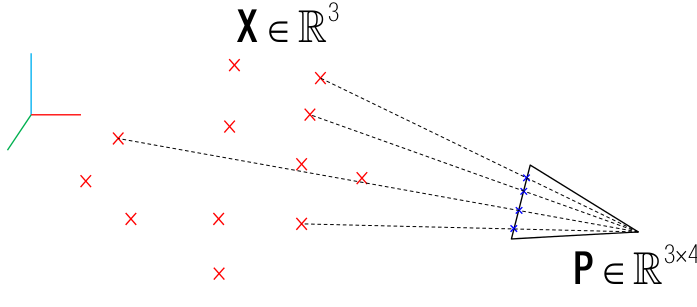
\includegraphics[width=\linewidth]{pnp.png}
  \caption{Perspective-n-Point Setup}
  \label{fig:pnp}
\end{figure}

Although there are multiple approaches to solving this problem, only the standard algorithm is briefly explained here for brevity.
\begin{description}
\item \textbf{Linear Standard Method:} As suggested by its name, this method assumes linear relationship among the variables and devises a solution based on this assumption. According to this method, solving PnP translates to finding solution to the following relation: \newline

\begin{equation}\label{pnpsolveeq}
\begin{bmatrix}
0_{1\times4} & -X^{T} & vX^{T}\\
X^{T} & 0_{1\times4} & uX^{T}\\
-vX^{T} & uX^{T} & 0_{1\times4}
\end{bmatrix}
\begin{bmatrix}
P_{1}^{T}\\
P_{2}^{T}\\
P_{3}^{T}
\end{bmatrix}
= 0
\end{equation}
Where $x = \begin{bmatrix}
u&
v&
1
\end{bmatrix}^T$, and $P_{i}$ is the $ith$ row of camera projection matrix $P$. Now, given that $P$ is estimated, $R$ and $t$ is further computed as follows:
\begin{equation}\label{pnpeq}
R' = K^{-1}P_{1:3}
\end{equation}

\begin{equation}\label{pnpeq2}
R = UV^{T}
\end{equation}

\begin{equation}\label{pnpeq3}
t = K^{-1}P_{4} / \sigma_{1}
\end{equation}

where $R'=UDV^{T}$ and $D = diag(\sigma_{1},\sigma_{2},\sigma_{3})$. Note that equation \eqref{pnpeq2} is used to enforce orthogonality constraint of rotation matrix $R$.
\end{description}

\subsection{Random sample consensus} Random sample consensus (RANSAC) is an outlier detection method used to estimate parameters of a mathematical model from a set of observed data that contains outliers, when outliers are to be accorded no influence on the values of the estimates \cite{ransac}. We use this method for fitting a line such that it passes through a maximum number of points.

There are several other methods apart from RANSAC, such as the least squares method. For line fitting, we are given with a set of $x$ and $y$ points that lie close to the line. Our goal is to fit a line represented by a three parameter family of homogeneous points on the line, $e$, $f$, and $g$. This can be written as a linear combination where each row contains the homogeneous coordinates of the point, which is repeated $N$ times, i.e., number of points, as shown in equation (\ref{least-squares}). This can be solved using SVD where we decompose the vector $A$ into a three column vector $\begin{bmatrix} V_{1} & V_{2} & V_{3} \end{bmatrix}$. The last column of this vector gives us the solution.

However, this method is extremely sensitive to outlier points and can thus fit a line that is off course. This is because the cost function we are minimizing is the distance between the point and the line. This is shown in Figure \ref{fig:least-squares}.

\begin{figure}[!ht]%
    \centering
    \subfloat[Outlier absent]{{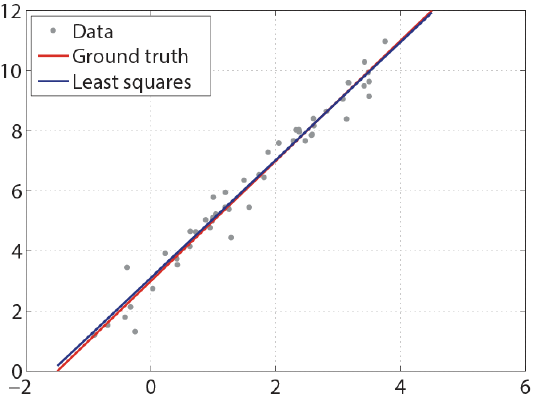
\includegraphics[width=6cm]{line-fitting-ls-correct.png} }}%
    \qquad
    \subfloat[Outlier present]{{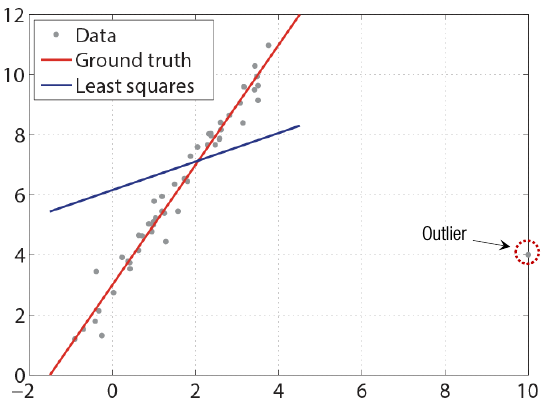
\includegraphics[width=6cm]{line-fitting-ls-nums.png} }}%
    \caption{Least squares method}%
    \label{fig:least-squares}%
\end{figure}

\begin{equation}\label{least-squares}
E = \left \| \begin{bmatrix}
 x_{1}  & y_{1} & 1 \\
 .  & . & . \\
 .  & . & . \\
 .  & . & . \\
 x_{N}  & y_{N} & 1
\end{bmatrix} \begin{bmatrix}
e\\ \\
f\\ \\
g
\end{bmatrix} \right \|^{2} = \left \| Ax \right \|^{2}
\end{equation}

RANSAC solves this problem by removing outlier points if its error is greater than a certain threshold $\varepsilon$. The strategy here is to find a model that accords with the maximum number of samples. It operates by randomly sampling points that belong to a group. If $p$ is the probability of each point belonging to a group, then $p^{k}$ is the probability of $k$ times while remaining in the same group. As we want this probability to be high, we sample only two points. Next, we find the number of inlier points. This procedure is repeated until we find a set of points that contain the maximum number of inliers. The probability of choosing an inlier is given by:

\begin{equation}\label{prob-inlier}
w = \frac{\# \ of \ inliers}{\# \ of \ samples}
\end{equation}

This refined approach gives us much better immunity against outliers, as shown in Figure \ref{fig:ransac}.

\begin{figure}%
    \centering
    \subfloat[]{{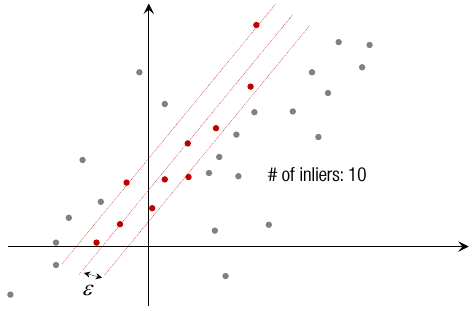
\includegraphics[width=6cm]{outlier-ransac-2.png} }}%
    \qquad
    \subfloat[]{{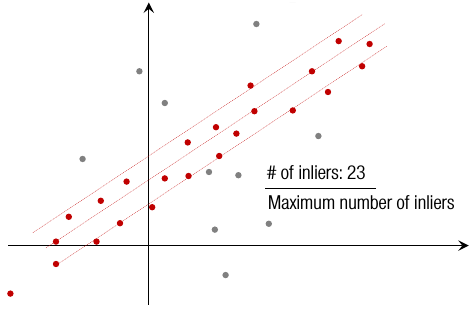
\includegraphics[width=6cm]{outlier-ransac-final.png} }}%
    \caption{RANSAC method}%
    \label{fig:ransac}%
\end{figure}

\section{Proposed Approach}

The steps involved in the reconstruction process are as follows.

\subsection{Feature Matching} As explained above, a set of 2D point correspondences are required for various steps. First, two video frames are selected and 2D point correspondences are found using an automated algorithm. Specifically, we used SIFT (Scale Invariant Feature Transform) \cite{SIFT} algorithm for computing features across the two images. These features are matched using nearest neighbor technique (L2 norm is used as a distance metric). Examples are shown in Figure \ref{fig:castle}(c) and \ref{fig:car}(c).

\subsection{Fundamental Matrix Estimation} Feature matching algorithms often match wrong correspondences that adds an overhead for removing outliers points i.e false correspondences. Due to this reason, the 8 point algorithm is used in conjunction with random sample consensus (RANSAC). Precisely, the algorithm proceeds as follows:

\begin{enumerate}
\item Pick any 8 random sample points and assume them to be correct correspondences.
\item Run 8 point algorithm (detail in section \ref{8pointsec}) using the points picked in previous step.
\item Count the number of inliers.
\item Go to step 1 unless number of pre-specified iterations are completed.
\end{enumerate}

Finally, the fundamental matrix $F$ having the most inliers is assumed to be the correct one.
\subsection{Pose Estimation} Once the fundamental matrix $F$ is computed, equation \eqref{essfund} is used to compute essential matrix to ultimately compute four possible camera projection matrices. The ambiguity among the four matrices is resolved through point triangulation i.e checking which $P$ among the four projects \textit{all} 2D image points in-front of them ($z >= 0$).

\subsection{Triangulation} Now that we have point correspondences $x_{1}, x_{2}, \ldots , x_{n}$ (corresponding to the same 3D point in real scene) and camera matrices $P_{1}, P_{2}, \ldots , P_{n}$ computed for each image $I_{1}, I_{2}, \ldots I_{n}$, we can use equation \eqref{lintri} to solve for $X$.

We use singular value decomposition of the left matrix to get $UDV^{T}$, where the last column of $V$ is the back-projected 3D point.

\subsection{Perspective-n-Point} SIFT features of the next frame are computed again to ultimately match 2D feature coordinates with 3D points already triangulated (in previous step).\newline
Now that we have a set of $X \leftrightarrow x$ correspondences and camera intrinsic parameters $K$, we can use equation \eqref{pnpsolveeq} to solve for camera projection matrix $P$. And we do so using, again, singular value decomposition as explained in section \ref{ssec:num1}.

\section{Implementation} Our implementation can be broadly divided into the following two modules:
\begin{description}
\item \textbf{Video Transfer} Video stream is captured from an Android smartphone over a localhost connection, using an Android application named \verb|IP Webcam|, which is then transfered to a host computer. To extract individual frames, \verb|FFmpeg| is used.
\item \textbf{Structure from Motion Pipeline} The source code for structure from motion pipeline is written in \verb|Python|. We primarily used the \verb|OpenCV| library for most of our computational tasks. The plotting is done using \verb|Matplotlib|.

An algorithmic description of our process is given below. All these step are performed using the \verb|OpenCV| library:

\begin{enumerate}
\item \textbf{Feature Matching} Given two video frames, their 2D point correspondences are found using the SIFT algorithm. The \\ \verb|detector.detectAndCompute| function serves this purpose.

\item \textbf{Fundamental Matrix Estimation} The output from our previous step is refined using the 8 point algorithm, which gives us the fundamental matrix with most inliers. This function is named \verb|cv2.findFundamentalMat| in \verb|OpenCV|.

\item \textbf{Pose Estimation} To estimated the camera pose, we use the \verb|cv2.recoverPose| function. The ambiguity among the output is resolved using point triangulation.

\item \textbf{Triangulation} Using the \verb|cv2.triangulatePoints| function, we apply SVD on our previous output to get $UDV^{T}$, where the last column of $V$ is the back-projected 3D point.

\item \textbf{Perspective-n-Point} In the last step, we estimate the camera projection matrix $P$ using the \verb|cv2.solvePnPRansac| function.

\end{enumerate}
\end{description}

\subsection{Web Interface}
The front-end web interface for our project is made using the Django web framework. It allows the user to upload image sequences (JPG, PNG format) which are sent to the server for 3D reconstruction. Once the reconstruction process is finished, the result is visualized using the \verb|Three.js| JavaScript library. We use Google Cloud for hosting the website, which can be accessed through a public IP address.

There are three pages provided by the website, namely, the Home page, How it Works page, and the Team page.

\subsubsection{Back-End Infrastructure}
To keep track of user images, we store the data in an SQLite database. It consists of the following fields: \verb|session_id|, \verb|file_name|, \verb|file_size|, \verb|file_format|, and \verb|date_created|. The actual image data is stored in a separate directory and \verb|file_name| is be used to query the image. For loading the images relevant to a particular user, the \verb|session_id| value is used, which has a unique value for each user session.

\subsubsection{Front-End Design}
A screenshot of our project's homepage is provided in Figure \ref{fig:homepage}.

\begin{figure}[H]
  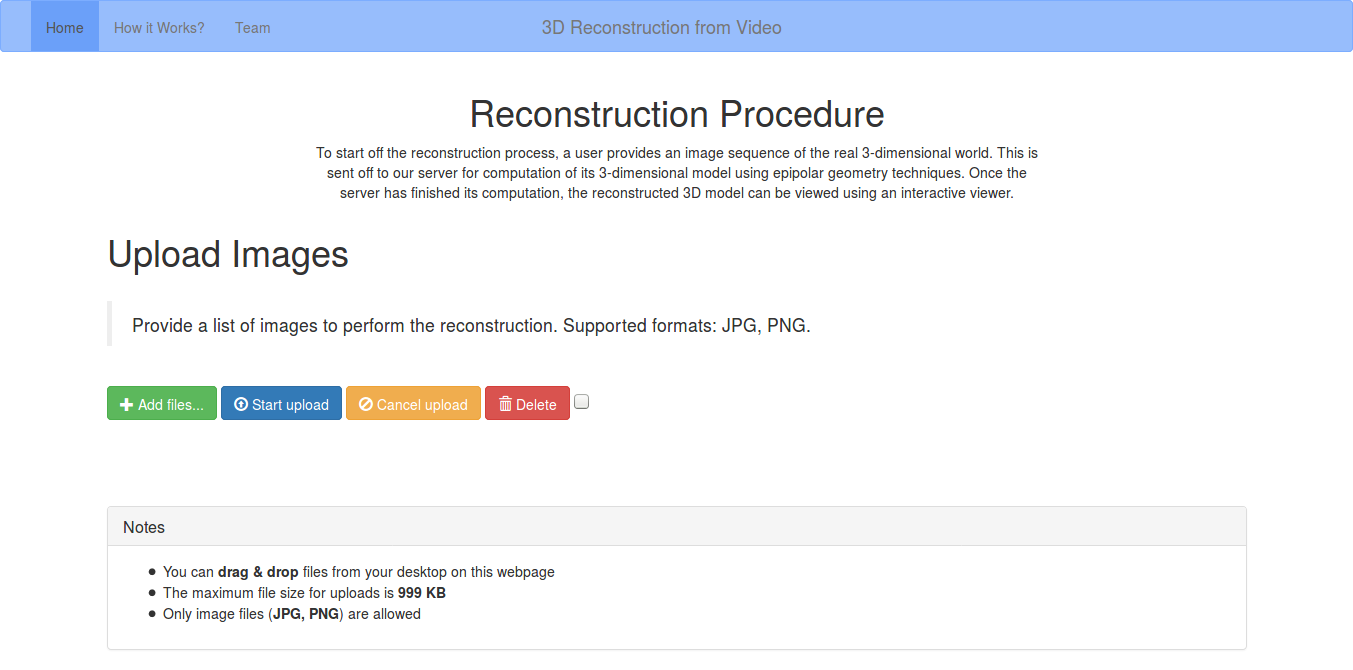
\includegraphics[width=\linewidth]{front-end.png}
  \caption{Homepage}
  \label{fig:homepage}
\end{figure}

\subsubsection{Point Cloud Visualization}
As mentioned earlier, we make use of the \verb|Three.js| JavaScript library for visualizing the end result, which is in the form of a point cloud. The library supports adding colors to the point cloud, and provides further controls for interacting with the points, such as zooming in and out, rotating and moving the camera. Figure \ref{fig:result} shows this in action.

\begin{figure}[H]
  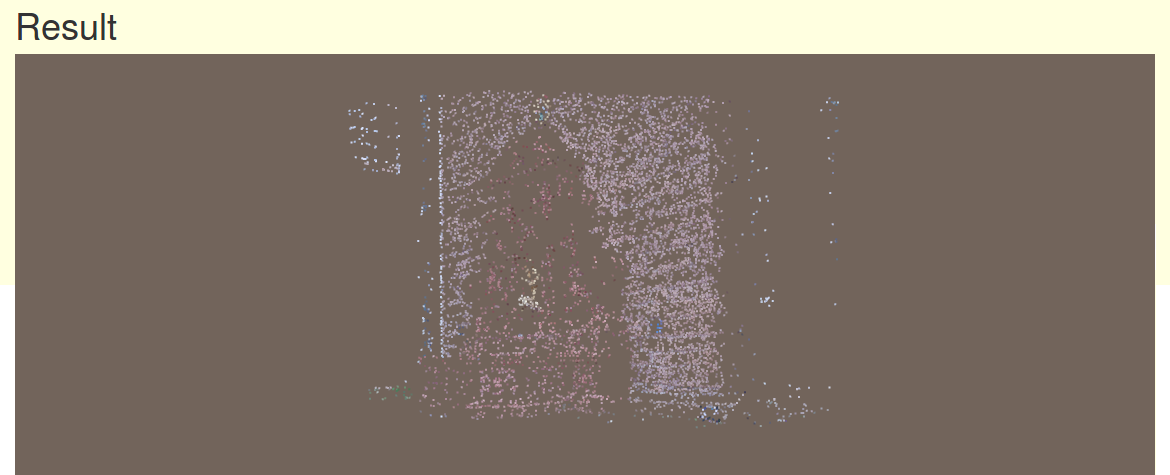
\includegraphics[width=\linewidth]{result.png}
  \caption{Interactive Point Cloud Viewer}
  \label{fig:result}
\end{figure}


\section{Results and Discussion}
We applied the above mentioned techniques to a variety of videos (shot in 30 frames per second) in both indoor and outdoor environments. The qualitative results are shown in figure \ref{fig:castle} and \ref{fig:car}.

For evaluating our system, we calculate the re-projection error and number of SIFT keypoint matches, as shown in Table \ref{tab:matches}.

\begin{table}[H] % Add the following just after the closing bracket on this line to specify a position for the table on the page: [h], [t], [b] or [p] - these mean: here, top, bottom and on a separate page, respectively
\centering % Centers the table on the page, comment out to left-justify
\begin{tabular}{l c c c c c} % The final bracket specifies the number of columns in the table along with left and right borders which are specified using vertical bars (|); each column can be left, right or center-justified using l, r or c. To specify a precise width, use p{width}, e.g. p{5cm}
\toprule % Top horizontal line
& \multicolumn{3}{c}{Statistics} \\ % Amalgamating several columns into one cell is done using the \multicolumn command as seen on this line
\cmidrule(l){2-4} % Horizontal line spanning less than the full width of the table - you can add (r) or (l) just before the opening curly bracket to shorten the rule on the left or right side
Dataset & SIFT keypoints count & Inliers count & Ratio\\ % Column names row
\midrule % In-table horizontal line
Castle (frame 19) & 4000 & 1221 & 0.30525\\ % Content row 1
Castle (all frames) & 4000 & 1054.5925 & 0.26364\\ % Content row 2
Car (frame 6) & 4000 & 2271 & 0.56775\\ % Content row 3
Car (all frames) & 3935.9009 & 1239.9369 & 0.31503\\ % Content row 4
Building (all frames) & 3606.4721 & 1382.4163 & 0.38331\\ % Content row 5
Boot (all frames) & 744.3125 & 54.0625 & 0.07258\\ % Content row 6
\midrule % In-table horizontal line
\midrule % In-table horizontal line
Average & 3381.1142 & 1203.8347 & 0.31792\\ % Summary/total row
\bottomrule % Bottom horizontal line
\end{tabular}
\caption{Number of matches} % Table caption, can be commented out if no caption is required
\label{tab:matches} % A label for referencing this table elsewhere, references are used in text as \ref{label}
\end{table}

The table above lists two important entities; number of SIFT keypoint matches and the inliers count. These values can be used as an evaluation metric for our system, as their ratio should approach $1$, which will give us better results.

Another evaluation metric we use is the re-projection error, which is a numeric value corresponding to the image distance between a projected point and a measured one. Minimizing the re-projection error can be used for estimating the error from point correspondences between two images. This is shown below in Table \ref{tab:error}.

\begin{table}[H] % Add the following just after the closing bracket on this line to specify a position for the table on the page: [h], [t], [b] or [p] - these mean: here, top, bottom and on a separate page, respectively
\centering % Centers the table on the page, comment out to left-justify
\begin{tabular}{l c c c c c} % The final bracket specifies the number of columns in the table along with left and right borders which are specified using vertical bars (|); each column can be left, right or center-justified using l, r or c. To specify a precise width, use p{width}, e.g. p{5cm}
\toprule % Top horizontal line
Dataset & Average error\\ % Column names row
\midrule % In-table horizontal line
Castle (frame 19) & 308394.2187\\ % Content row 1
Castle (all frames) & 133857.5355\\ % Content row 2
Car (frame 6) & 60877.8515\\ % Content row 3
Car (all frames) & 569505.4980\\ % Content row 4
Building (all frames) & 3976174.3395\\ % Content row 5
Boot (all frames) & 42686.0363\\ % Content row 6
\bottomrule % Bottom horizontal line
\end{tabular}
\caption{Re-projection error} % Table caption, can be commented out if no caption is required
\label{tab:error} % A label for referencing this table elsewhere, references are used in text as \ref{label}
\end{table}

\begin{figure}[H]%
    \centering
    \subfloat[Input image]{{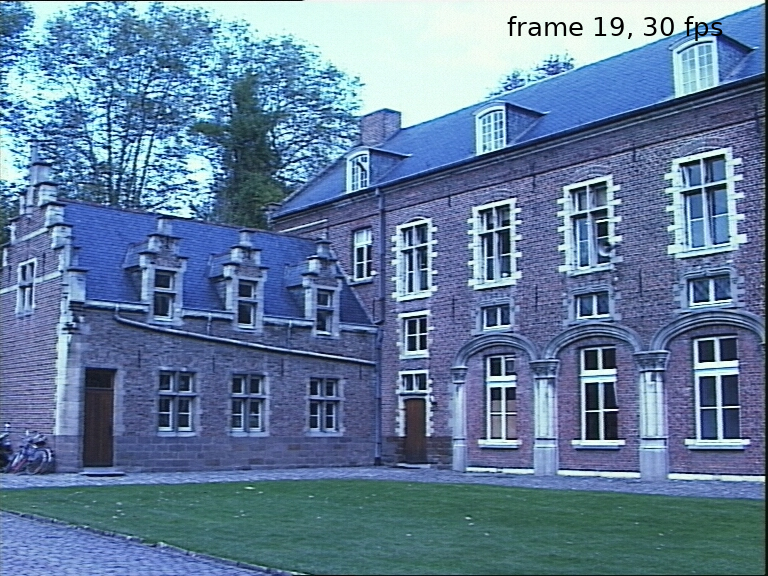
\includegraphics[width=6cm]{castle-019.jpg} }}%
    \qquad
    \subfloat[Rectified]{{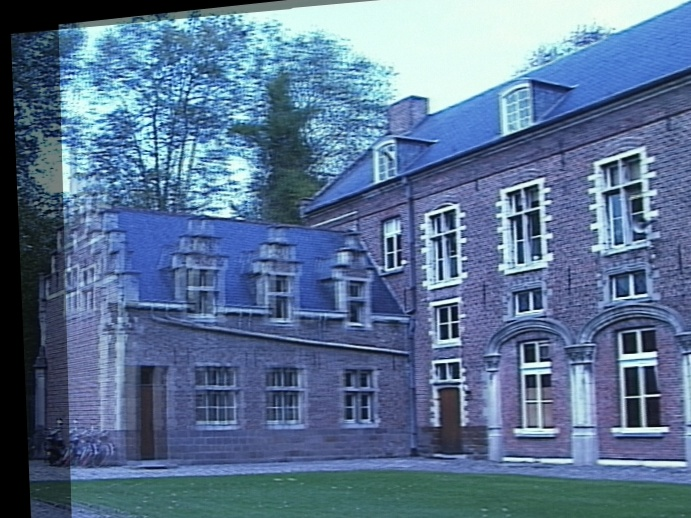
\includegraphics[width=6cm]{rectified-019.jpg} }}%
    \qquad
    \subfloat[SIFT keypoint matches]{{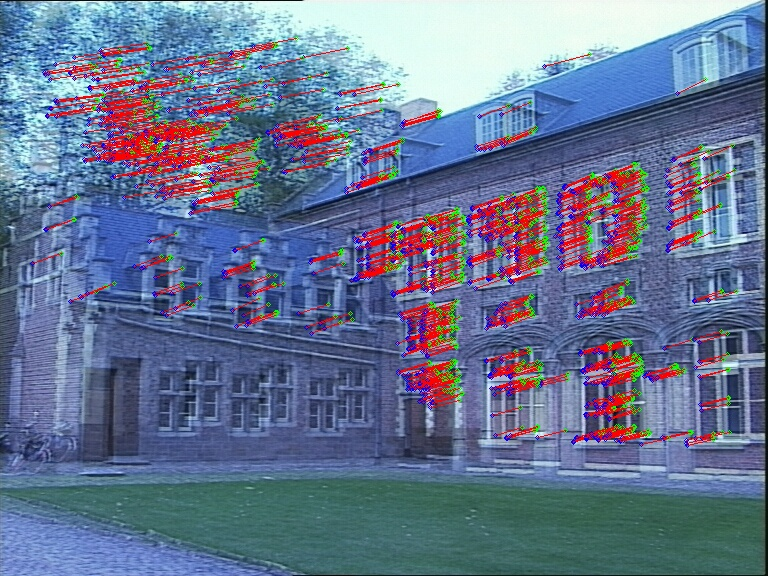
\includegraphics[width=6cm]{keypoint-matches-019.jpg} }}%
    \qquad
    \subfloat[Disparity map]{{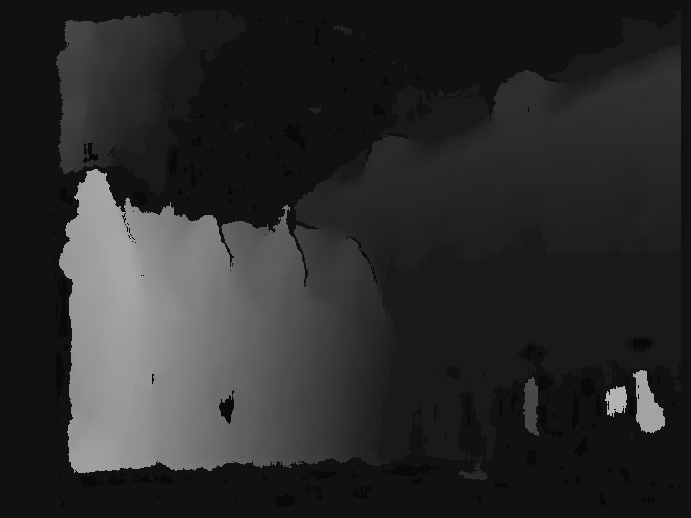
\includegraphics[width=6cm]{disparity-019.jpg} }}%
    \caption{Castle}%
    \label{fig:castle}%
\end{figure}

\begin{figure}[H]%
    \centering
    \subfloat[Input image]{{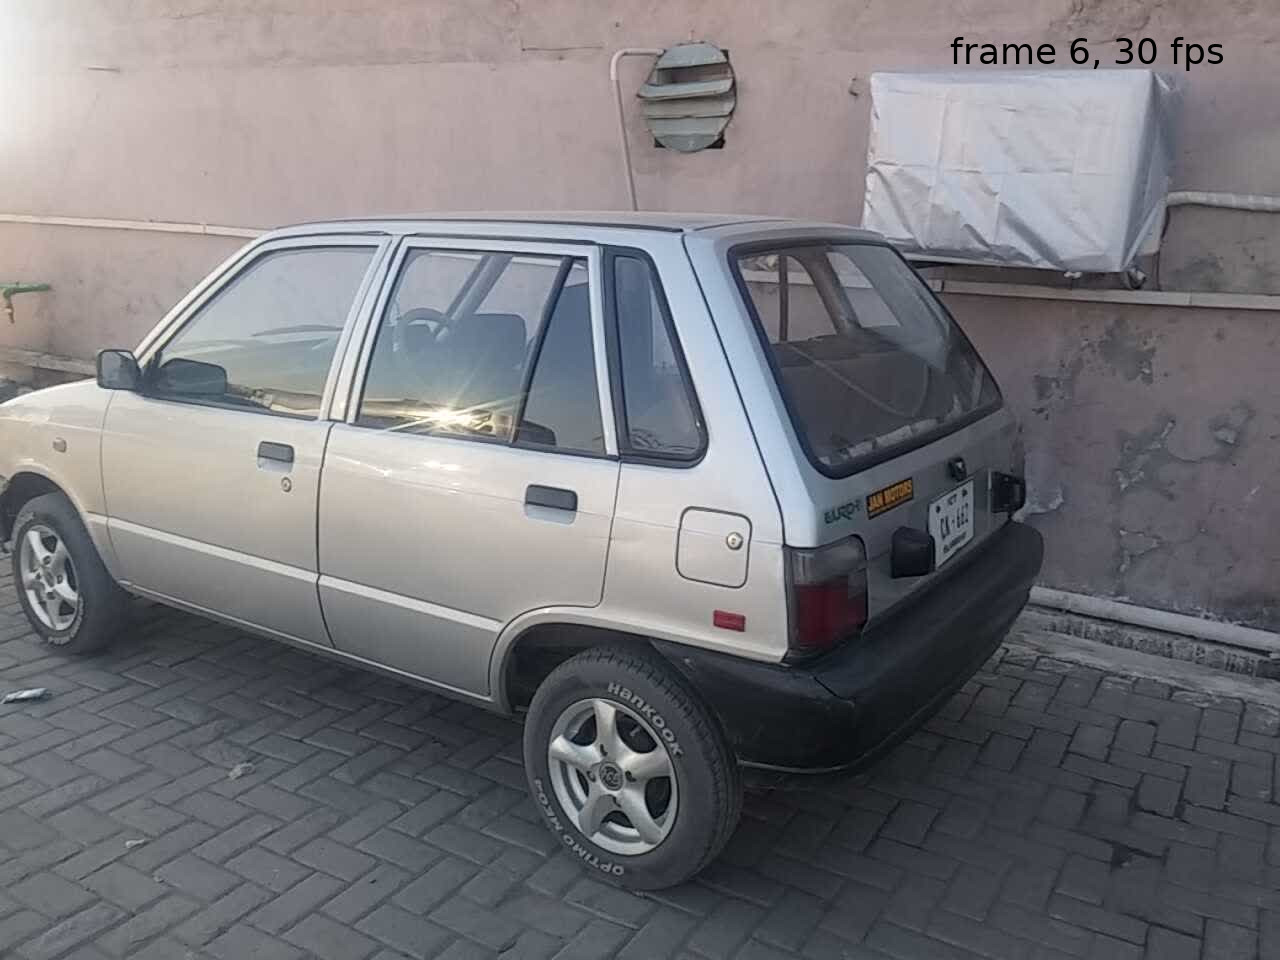
\includegraphics[width=6cm]{image-006.jpg} }}%
    \qquad
    \subfloat[Rectified]{{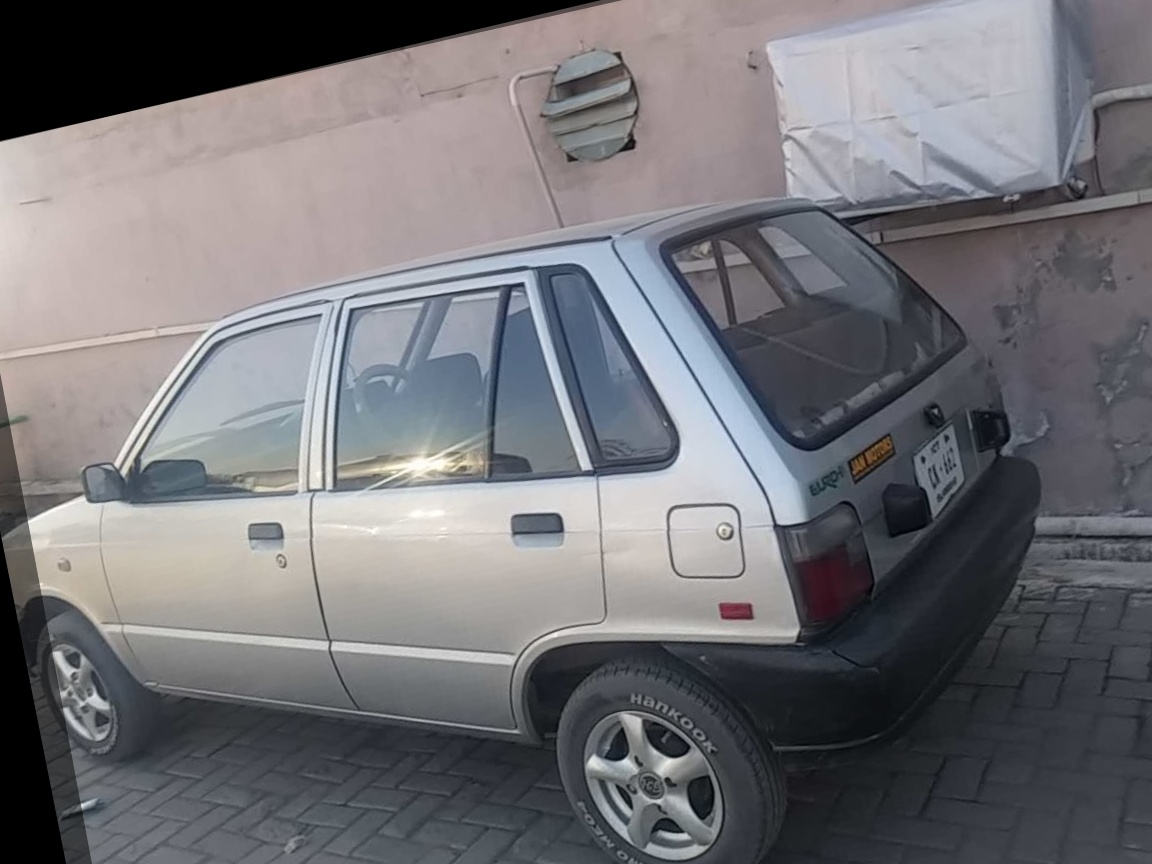
\includegraphics[width=6cm]{car-rectified-006.jpg} }}%
    \qquad
    \subfloat[SIFT keypoint matches]{{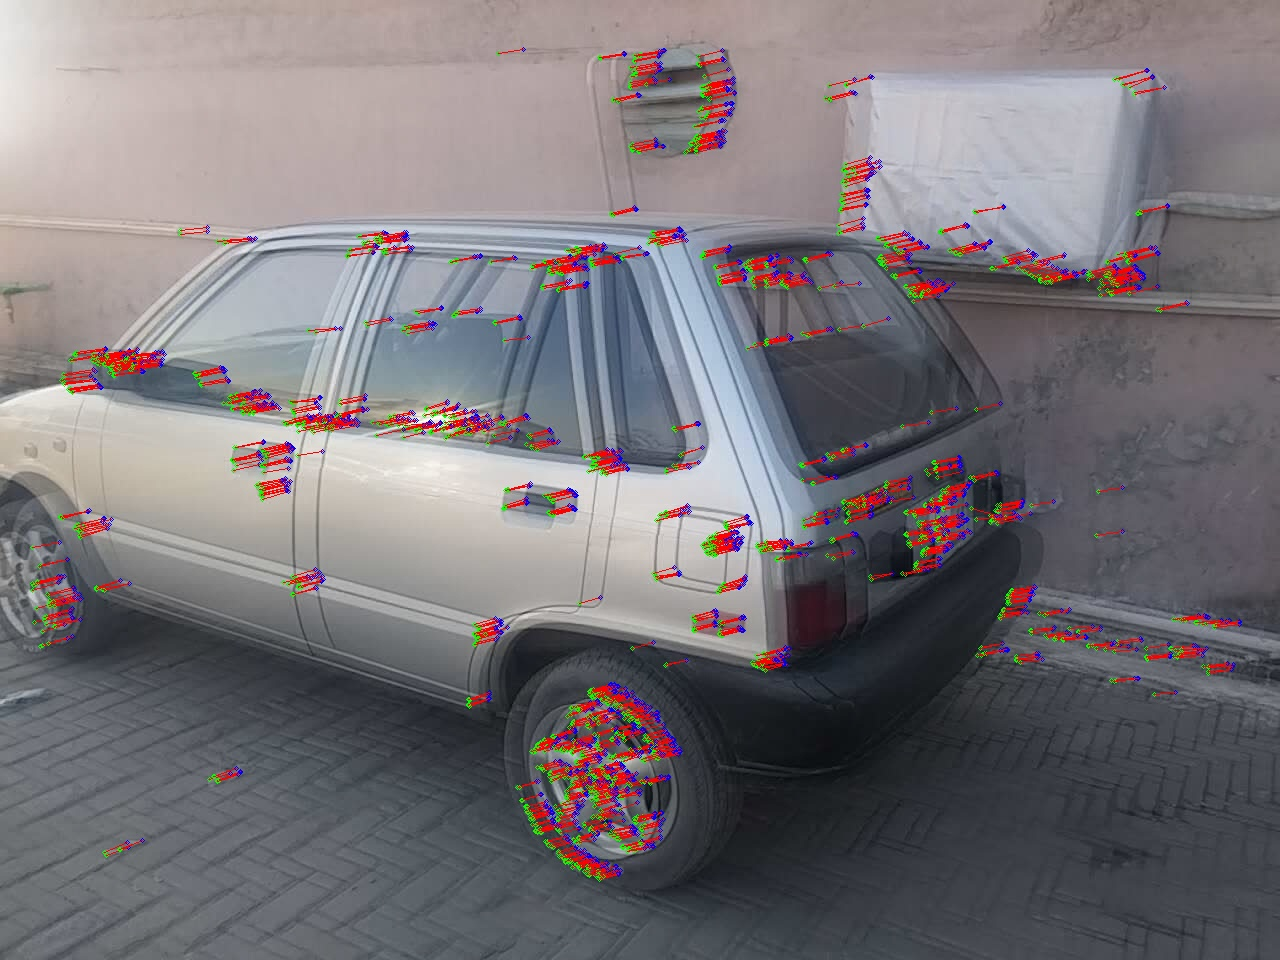
\includegraphics[width=6cm]{car-keypoint-matches-006.jpg} }}%
    \qquad
    \subfloat[Disparity map]{{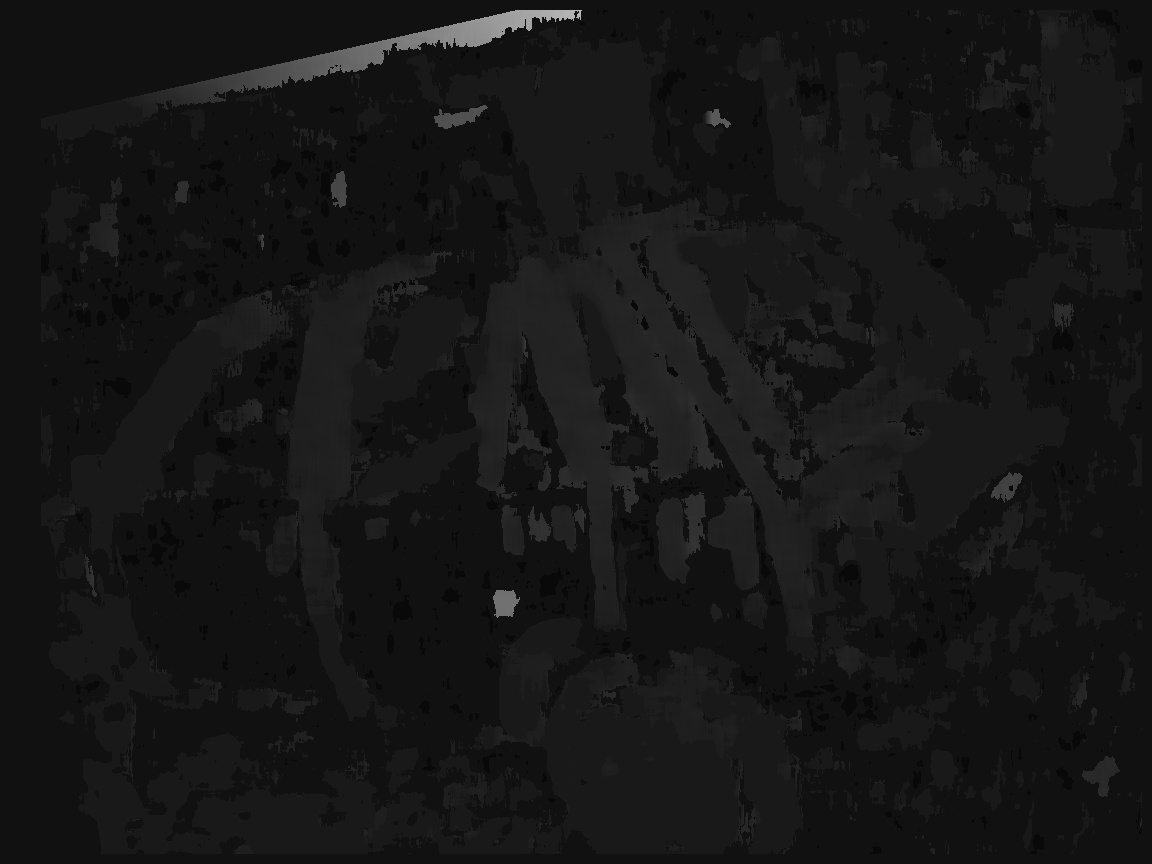
\includegraphics[width=6cm]{car-disparity-006.jpg} }}%
    \caption{Car}%
    \label{fig:car}%
\end{figure}
\section{Conclusions}
Using a monocular camera, we presented a system which takes input in the form of images and applies all the necessary steps for reconstructing a 3D model. The approach estimates camera pose, SIFT keypoint matches, and disparity map.

To allow for the correct fusion of resulting images and to better generalize our system, we calculate the re-projection error which allows us to evaluate our system. Our system does not require any initialization of scene structure and works for all input types, i.e., both outdoor and indoor environments.

A web interface was created which allows users to feasibly use our system. The resulting point cloud was visualized on our web page using a JavaScript viewer.

\newpage

% \bibliographystyle{APA}
\begin{thebibliography}{5}
\bibitem{photogrammetry}
Nuttens, Timothy, Alain De Wulf, Rudi Goossens, et al., ``Digital Photogrammetry Used for the 3D Reconstruction of the Walls Around the Acropolis of Titani (Greece)'', 2010.\\
\url{https://biblio.ugent.be/publication/1044358}

\bibitem{reconstruction steps}
Robert Collins, ``Stereo Reconstruction: Steps to General Stereo'', 2007.\\
\url{http://www.cse.psu.edu/~rtc12/CSE486/lecture21_6pp.pdf}

\bibitem{camera model}
Augusto Román, ``Multiperspective Imaging for Automated Urban Visualization'', 2006.\\
\url{https://graphics.stanford.edu/papers/aroman_thesis/UrbanMPI-thesis.pdf}

\bibitem{camera model2}
Hartley, Richard, and Andrew Zisserman, ``Multiple View Geometry in Computer Vision'', 2nd ed. Cambridge University Press, pp. 153-176, 2004.

\bibitem{pose estimation}
Darius Burschka, Elmar Mair, ``Direct Pose Estimation with a Monocular Camera'', 2017.\\
\url{https://arxiv.org/pdf/1709.05815.pdf}

\bibitem{section 9.1}
Hartley, Richard, and Andrew Zisserman, ``Multiple View Geometry in Computer Vision'', 2nd ed. Cambridge University Press, pp. 239-241, 2004.

\bibitem{section 9.6}
Hartley, Richard, and Andrew Zisserman, ``Multiple View Geometry in Computer Vision'', 2nd ed. Cambridge University Press, pp. 257, 2004.

\bibitem{fundamentalcorrespondingcondition}
Hartley, Richard, and Andrew Zisserman, ``Multiple View Geometry in Computer Vision'', 2nd ed. Cambridge University Press, pp. 247, 2004.

\bibitem{triangulation}
Richard Hartley, Peter Sturm, ``Triangulation'', Springer-Verlag, 970, pp. 190-197, 1995, Lecture Notes in Computer Science (LNCS).\\
\url{http://www.springerlink.com/content/7027546l38383587}

\bibitem{pnpref}
Xiao-Shan Gao, Xiao-Rong Hou, Jianliang Tang and Hang-Fei Cheng, ``Complete solution classification for the perspective-three-point problem'', in IEEE Transactions on Pattern Analysis and Machine Intelligence, vol. 25, no. 8, pp. 930-943, Aug. 2003.\\
\url{http://ieeexplore.ieee.org/document/1217599}

\bibitem{SIFT}
D. G. Lowe, ``Object recognition from local scale-invariant features'', Proceedings of the Seventh IEEE International Conference on Computer Vision, Kerkyra, 1999, pp. 1150-1157 vol.2.\\
\url{https://ieeexplore.ieee.org/document/790410/}

\newpage

\bibitem{8point}
R. I. Hartley, ``In defense of the eight-point algorithm'', in IEEE Transactions on Pattern Analysis and Machine Intelligence, vol. 19, no. 6, pp. 580-593, Jun 1997.
In Defence of the 8-point Algorithm, Richard I. Hartley, 1997\\
\url{https://ieeexplore.ieee.org/iel1/34/13258/00601246.pdf}

\bibitem{ransac}
Yaniv Z. ``Random Sample Consensus (RANSAC) Algorithm, A Generic Implementation'', Oct. 2010.\\
\url{http://www.insight-journal.org/browse/publication/769}

\end{thebibliography}
\newpage
\appendix
\section{Singular Value Decomposition for Solving $Ax = 0$}
Often, we need to solve $Ax = 0$, but due to noise in the data, this equation does not exactly hold in practice. Due to which the problem reduces to
\begin{equation}
\underset{x}{min}
\begin{Vmatrix}
Ax
\end{Vmatrix}
\end{equation}
Thus, we try to find, not the exact nullspace of A, but rather a vector $x$ close to nullspace. This vector corresponds to the row-space vector of A which contributes minimally in matrix $A$ construction. Thus
\begin{equation}
x = V(:,end)
\end{equation}
Where
\begin{equation}
A = UDV^{T}
\end{equation}
\end{document}
